\documentclass[10pt,journal,compsocconf]{IEEEtran}

\usepackage{hyperref}
\usepackage{graphicx}
\usepackage{subcaption}
\usepackage{siunitx}
\usepackage{biblatex}
\usepackage{mathtools}
\usepackage[font=small]{caption}
% \usepackage{subcaption}

\usepackage{fancyhdr}
\pagestyle{fancy}
\cfoot{\thepage}

\title{CS-454 Final Project (N-Body problem) -- Fall 2023}
\author{
  Sepehr Mousavi (Sciper: 338673)
}
\date{\today}
\newcommand{\code}[1]{\texttt{#1}}

\begin{document}

\maketitle

\section{Introduction}

The provided sequential codes for solving the N-body problem have been modified to take advantage of multiple processors using the MPI library for the Barnes-Hut algorithm and using GPUs for the particle-particle method. Prior to the parallelizations, the sequential codes are profiled to get an estimation of the fraction of the parallelizable part of the code. The modified codes have been executed to measure the performance of the implementations with multiple cores and different GPU grid and block sizes. Along with this report, you will find a compressed archive file containing all the \texttt{C++} and CUDA codes, make files, slurm jobs, and shell scripts for reproducing the experiments. The codes for producing the visualizations are included in \code{visualizations.ipynb}.

All the experiemnts are done using the \texttt{data/galaxy.txt} dataset and with 20 iterations. In the rest of the document, $N$ represents the number of particles considered from this dataset.

\section{Profiling of the sequential code}

The initial sequential codes are cleaned, commented, and improved, and the input arguments of the main executable are extended so that the method can be picked during runtime. The codes are adapted to \texttt{C++} and some standard library classes are used. The input/output of the code is also modified to facilitate the post-processing of the results. However, the logic of the initial codes are not changed except for the removal of the \texttt{compute\_bh\_force} function in the Barnes-Hut algorithm. This function computes the force of the particles on themselves, and removing it would not change the results.

The cleaned sequential codes are used for profiling and as the base for the other parts of the project. They are located in \texttt{./src/seq}. Both methods are profiled with \texttt{gprof} and \texttt{perf} and the results are available in \texttt{./results/20231230161253} and \texttt{./results/20231230161348}. The scripts in \texttt{./scripts/seq-profiling.sh} and \texttt{./scripts/job-seq-profiling.sh} are used for the profilings. For both methods, the results of \texttt{perf-stat} indicate that only 0.13\% of the cache loads have been missed.

The results of \texttt{gprof} for the Barnes-Hut method indicate that around 78\% of thetotal execution time is consumed by the \texttt{compute\_force\_particle} and the\texttt{compute\_force\_in\_node} functions, and around 5\% by \texttt{move\_all\_particles}.The results of \texttt{perf-report} indicate that around 73\% of the total execution timeis spent in \texttt{compute\_force\_in\_node} and around 14\% in \texttt{move\_all\_particles}.The parallelizable fraction of the code is therefore approximated as 85\%. It is notable thatthis number is an over-estimation since insertion of the particles in \texttt{move\_all\_particles}will not be targeted for parallelization in the taken approach.

Not much can be inferred from the results of \texttt{gprof} and \texttt{perf-report} for the brute force method since it is comprised of only 3 functions.

\section{Parallelization of the Barnes-Hut algorithm with MPI}

The parallelized version of the Barnes-Hut algorithm is available in \texttt{./src/mpi}. The computation of forces and changes in velocity and positions are targeted for this parallelization. Each particle is assined to a process based on its identifier. The rank of the processor is determined as $\text{rank}_p = (\text{id}_p - 1) \% \text{n}$, where $n$ is the total number of the processors and $\%$ represents the modulo operator. Hence, a \texttt{prank} member is added to the \texttt{particle} struct and is assigned in \texttt{read\_test\_case}. With this, in \texttt{compute\_force\_in\_node}, the forces are computed only if the particle is assigned to the processor. Similarly, the computation of the new velocities and positions in \texttt{move\_particle} is also only done if the particle is assigned to the processor. In order to separate this step with the construction of the new Barnes-Hut tree based on the new positions, two functions are introduced: \texttt{reassign\_all\_particles} and \texttt{reassign\_particle}, which are invoked only after the communication of the computations with the other processors is done using the \texttt{communicate} function.

In \texttt{communicate}, the new velocities and positions of the assigned particles along with their identifiers are packed in three long vectors, and are broadcasted to the other processes using \texttt{MPI\_Ibcast}. The new velocities and positions of the other particles are received from the other processes and are unpacked to update the particles.

In a failed attempt to benefit from computation-communication overlapping, another approach has also been tried for communications. In this approach, the computed forces of the particles are sent immediately after they are computed, one by one, and are expected by the other processors only before computation of the new positions. Although the communication of the forces are overlapped with the computation of the forces of the other particles, this approach performs very poorly because of the large number of communication requests. In each iteration, $O(N)$ communications are requested, compared to only $O(n)$ communications in the other approach. Another possible implementation is using \texttt{MPI\_Allgather} or one of its alternatives to transfer the computations to one array for all particles in all processes.

\subsection{Computational complexity}

Broadcasting in Open MPI is implemented using binominal trees, which has a complexity of order $O(M \log n)$ for a vector of length $M$. In the presented implementation, two vectors of length $3 \frac{N}{n}$ and one vector of length $\frac{N}{n}$ are broadcasted by each processor, which gives an overall communication complexity of $O(n \times \frac{N}{n} \log n) = O(N \log n)$ with fixed number of iterations. The packing and unpacking of the buffers are dominated by the exchange of the messages.

Since forces from the whole system are computed for only $\frac{N}{n}$ particles by each process,the algorithmic complexity of the computations scales down from $O(N \log N)$ in the sequential code to $O(\frac{N}{n} \log N)$. However, the complexity of \texttt{create\_bh\_tree} remains the same sicne this part of the code is not parallelized.

\subsection{Results}

A strong scaling and a weak scaling are performed to evaluate the performance of the code with multiple processors. For the strong scaling, we fix the size of the problem and launch the code with different number of processors $n$. For the weak scaling, we tend to keep the computational complexity of the problem fixed, and hence increase $N$ and $n$ at the same time. The pairs ($n$, $N$) for achieving this are: (1, 964), (2, 1770), (4, 3274), (8, 6081), (16, 11350), (32, 21268), and (64, 40000), which all result in the same computational complexity.

This process is repeated 10 times to mitigate the randomness that can happen in the processors. In the strong scaling, the speedup with $n$ processors in experiment $i$ is calculated by $S^{(i)}_{strong}(n) = t^{(i)}_1 / t^{(i)}_n$, where $t^{(i)}_n$ is the measured time in experiment $i$ with $n$ processors. Similarly, the efficiency in the weak scaling is calculated by $E^{(i)}_{weak}(n) = S^{(i)}_{weak}(n) / n = t^{(i)}_1 / t^{(i)}_n$. Figure \ref{fig:strongscaling} shows the medians of speedups across all the 10 experiments along with their 90\% confidence intervals for different problem sizes. The ideal speedup and the upper bound from Amdahl's law with $p=85\%$ are also depicted. In Figure \ref{fig:weakscaling}, the medians of the measured efficiencies across all experiment are plotted along with their 90\% confidence intervals. The ideal efficiency and the upper bound from Gustafon's law with constant parallelization ratio $p(N)=85\%$ is also depcited. In both figures, the discrepency with the theoretical upper bounds is plotted in the right part.

\begin{figure*}[ht]
  \centering
  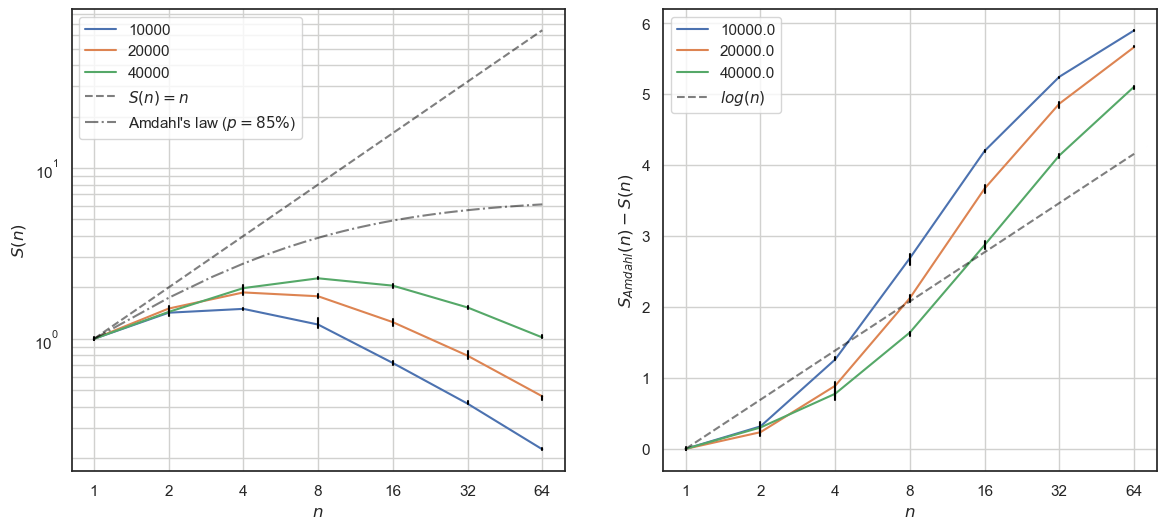
\includegraphics[width=.9\textwidth]{img/strongscaling.png}
  \caption{Empirical strong scaling speedup with different problem sizes aggregated over 10 experiments.}
  \label{fig:strongscaling}
\end{figure*}

\begin{figure*}[ht]
  \centering
  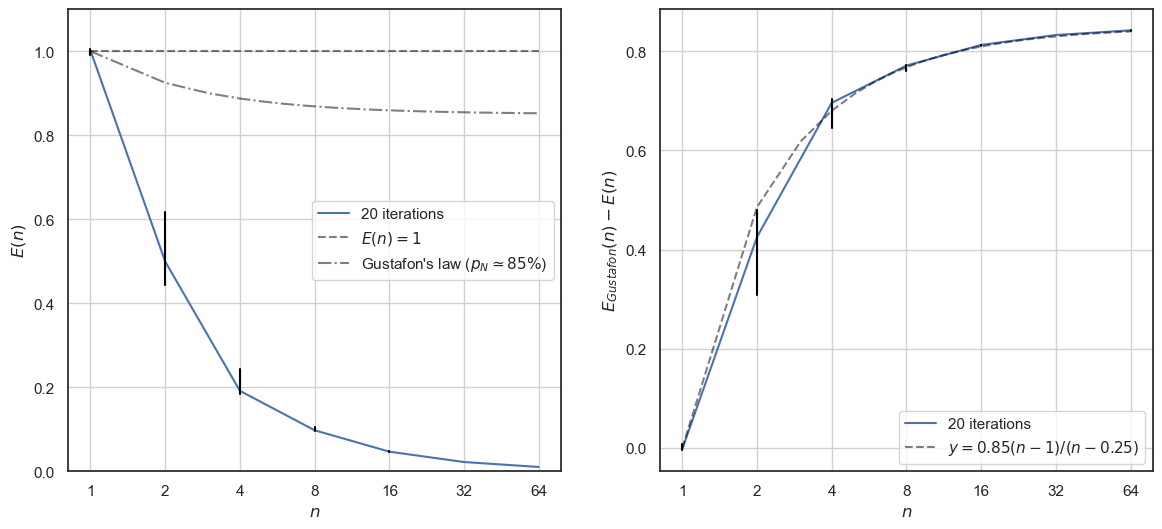
\includegraphics[width=.9\textwidth]{img/weakscaling.png}
  \caption{Empirical weak scaling efficiency aggregated over 10 experiments.}
  \label{fig:weakscaling}
\end{figure*}

\subsection{Discussion}

The theoretical speedup from Amdahl's law with an upper-estimation of the parallelizable fraction of the code gives an upper-bound of 6 for the speedup with 64 processors, which indicates that this parallelization approach does not scale well with many processors for a fixed-size problem. The empirical results in Figure \ref{fig:strongscaling} show even worse speedups with a maximum speedup of ~2 with 8 processors. Regardless of the problem size, the performance is closer to Amdahl's law with only a few processors and starts decaying as more processors are used. This is because the communications start getting more and more expensive and eventually dominate the benefits in the computational costs when using more processors. Notice that the domination happens later for larger problems. With 64 processors, the speedup is 1 for 40000 particles, the same as using only one processor. For smaller problems (10000 and 20000 particles), the performance is even worse than using only one processor. The plot on the right side of Figure \ref{fig:strongscaling} shows the difference between the theoretical and the empirical speedups. We can observe that this difference behaves as $O(\log n)$ as $n$ gets larger. This observation is justified by the algorithmic complexities of the computation and the communication. In strong scaling, the complexity of the computation part for a fixed $N$ is $O(\frac{1}{n})$, and the complexity of the computation is $O(\log n)$. The computational cost is considered in Amdahl's law, and the difference comes largely from the cost of communication, which explains the observed behaviour.

The theoretical efficiency from Gustafon's law with an upper-estimation of the parallelizable fraction of the code gives an upper-bound of ~0.85 for the efficiency with many processors. Since the computational cost of the serial part of the code scales with the same order as the parallelizable part, it is viable to use the same fraction for all $N$. This can be confirmed by profiling the sequential code with different $N$.

The empirical results in Figure \ref{fig:weakscaling}, however, show a strong discrepency with the theoretical upper-bound. The efficiency already drops to 0.5 with only 2 processors and goes down to around zero with 64 processors. This behaviour originates mainly from the harsh increase in communication cost when using more processors. Let's characterize the cost of computations with $n$ processes by $W(n)$, the cost of communications by $C(n)$, and the execution time as $T(n) = O(W(n) + C(n))$. In weak scaling, $W(n)$ is kept constant, hence, we can say that $O(\frac{N}{n} \log N) = O(1)$ or $O(N \log N) = O(n)$. Using this simplification, we get

\begin{equation*}
  \begin{aligned}
    C(n) = & O(N \log n) = O(N [\log N + \log(\log N)]) \\
    & = O(N \log N) = O(n)
  \end{aligned}
\end{equation*}

which means that with more processors the cost of communications increases while the cost of computation per processor remains the same. The efficiency in weak scaling can be written as
\begin{equation*}
  E(n) = \frac{T(1)}{T(N)} = \frac{W(1)}{W(n) + C(n)} = 1 - \frac{C(n)}{W(n) + C(n)}.
\end{equation*}
The difference with Gustafon's law can thus be expressed as $\frac{O(n)}{O(n)}$. The right side of Figure \ref{fig:weakscaling} shows a possible function with this algorithmic behaviour along with the empirical results. As more processors are used, $C(n)$ becomes more and more dominating and the effect of $W(n)$ becomes insignificant.

\section{Parallelization of the Particle-Particle method with CUDA}
% TODO: Write


\section{Reproducibility}

All figures and numbers are generated from the experiment results that are included in \code{./results/}. In order to repeat the experiments and generate new plots, the following steps can be followed:
\begin{itemize}
    \item \code{\$ scripts/seq-profiling.sh}
    \item \code{\$ scripts/mpi-scaling.sh}
    \item \code{\$ scripts/cuda-xxxx.sh}
    \item Wait until the jobs are processed.
    \item \code{\$ mv -r ./output/* ./results/}
    \item Run \code{visualizations.ipynb}.
\end{itemize}

\section{Conclusion}

The performance of the Barnes-Hut algorithm for the N-body problem is evaluated with multiple processors by splitting the particles among the processors. Strong scaling shows that with the estimated parallelizable fraction, using many processors cannot theoretically be very beneficial, and the parallelization approach scales very poorly for fixed-size problems. However, for larger problems, it is possible to get speedups closer to Amdahl's law. Weak scaling was even more disappointing than the strong scaling, with an efficiency of ~0.5 with 2 processors and ~0.2 with 4 processors. This shows that increasing the problem size according to the available processors is not beneficial either. More sophisticated implementations of the algorithm or more sophisticated parallelization approaches are necessary for getting acceptable results. The lowest hanging fruit is parallelizing the tree construction as well as computation of forces and positions. A more complicated option is splitting the physical space among the processors with local information. With a smart implementation, each process will only need the information of particles in the nearby nodes, hence, less communications are needed. However, keeping the balance between the processors can be challenging with this appraoch.

\end{document}
